\documentclass{article}

\usepackage{graphicx}
\usepackage{cite}
\usepackage{hyperref}
\usepackage{amssymb}

\title{EEEE3087 Mobile technologies \\Coursework1}
\author{Yaowen Hu\\20495331}
% \date{\today}

\begin{document}

%%%%%%%%%%%%%%%%%%%%%%%%%%%%%%%%%%%%%%%%%%%%%%%

\begin{titlepage}
\begin{figure}
    \vspace{-4em}
    \centering
    
\includegraphics[width=0.9\textwidth]{images/logo.png}
\end{figure}

\vfill
\maketitle
\vfill

\centering{University of Nottingham}\\
\centering{\today}
\thispagestyle{empty}
\pagebreak
\end{titlepage}

%%%%%%%%%%%%%%%%%%%%%%%%%%%%%%%%%%%%%%%%%%%%%%%

\tableofcontents
\thispagestyle{empty}
\pagebreak

%%%%%%%%%%%%%%%%%%%%%%%%%%%%%%%%%%%%%%%%%%%%%%%

\begin{abstract}
\addcontentsline{toc}{section}{Abstract}
My abstract
\thispagestyle{empty}
\pagebreak
\end{abstract}

%%%%%%%%%%%%%%%%%%%%%%%%%%%%%%%%%%%%%%%%%%%%%%%

\section{Introduction and background research}

\pagestyle{plain}
\setcounter{page}{1}

\subsection{Introduction}
\textit{Orthogonal Frequency Division Multiplexing} (OFDM) is one of the most powerful modulation technique. It is designed for high-data-rate transmission. In general, it will convert a high-rate data stream into several low-rate data streams which can be transmitted in parallel\cite{RN79}. These streams or sub-carriers are orthogonal to each other, which means they don't interfere with each other, allowing multiple sub-carriers to be transmitted simultaneously over the same channel without causing interference.\\
OFDM is used in many different communication systems, including digital television, Wi-Fi, 4G and 5G LTE (Long-term Evolution) mobile networks, and \textit{Digital Subscriber Line} (DSL) modems over copper-based telephone access lines. Due to its excellent performance, OFDM has been standardized by IEEE into standards such as 802.11g and 802.11a\cite{RN79}.

\subsubsection{Principle of OFDM}
When the signal is transmitted in the air, it is very likely to be interfered and distorted by multi-path propagation which is shown in Figure \ref{fig:multipath propagation}. Hence, people are considering to transmit multiple non-interference sub-carriers which can be recovered easily by their orthogonality.

\begin{figure}[!h]
\centering
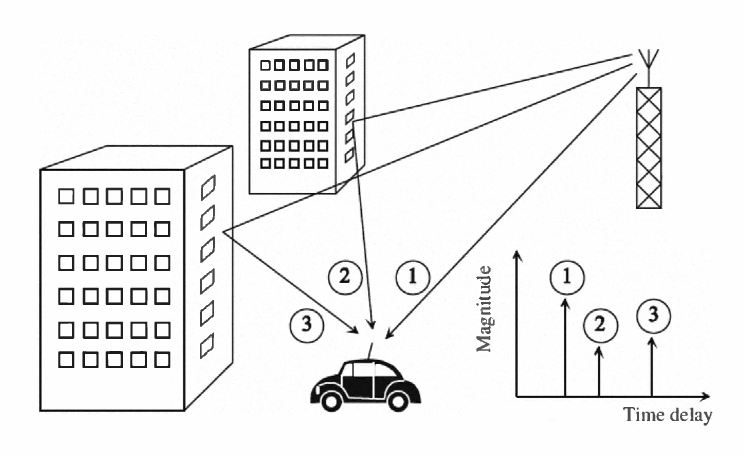
\includegraphics[width=0.8\textwidth]{images/multipath propagation.png}
\caption{\label{fig:multipath propagation}The multi-path propagation}
\end{figure}

In order to make there sub-carriers orthogonal to each other or not overlap each other in the frequency domain, the inner product of any two sub-carriers is zero. That is, in the time domain, the cross-correlation of any two sub-carriers is zero. As shown in the following Equation \ref{con:cc},

\begin{equation}
(f \star g) \triangleq \int_{-\infty}^{\infty} sub-carrier_1(t) \cdot sub-carrier_2(t)dt=0 \label{con:cc}
\end{equation}

At the receiver, the OFDM signal is first demodulated to recover the sub-carriers. Then, each sub-carrier is processed individually to recover the raw data. A parallel-serial converter is then used to convert the low-speed data stream to a high-speed data stream for use by the terminal.

\paragraph{Principle of OFDM}
Principle of OFDM

\subparagraph{Principle of OFDM}
Principle of OFDM

%%%%%%%%%%%%%%%%%%%%%%%%%%%%%%%%%%%%%%%%%%%%%%%

\section{BER analysis}
123\cite{RN79},dsad
sdasd

\section{Conclusion}
123


\bibliographystyle{IEEEtran}
\bibliography{exportlist}
\addcontentsline{toc}{section}{References}

\section{[Appendices]}
123


	
\end{document}